%% Support sites:
%% http://www.michaelshell.org/tex/ieeetran/
%% http://www.ctan.org/tex-archive/macros/latex/contrib/IEEEtran/
%% http://www.ieee.org/

% The testflow support page is at:
% http://www.michaelshell.org/tex/testflow/

\documentclass[journal]{IEEEtran}

\usepackage{blindtext}
\usepackage{graphicx}
\usepackage{cite}
\usepackage{float}
% correct bad hyphenation here
\hyphenation{op-tical net-works semi-conduc-tor}

%\renewenvironment{titlepage}
%{}

\title{Do No Harm: \\ Are Rainbow Colormaps Dangerous?}
\author{Derek~Miller \\ Brigham Young University}% <-this % stops a space


\begin{document}

% make the title area
\begin{titlepage}
%\maketitle
%\vspace*{\fill}

{\centering\LARGE{Do No Harm: Are Rainbow Colormaps Dangerous?} \\
\break
\small{Derek Miller---Brigham Young University} \\}
\begin{abstract}
This document addresses the controversies and contradictions
surrounding colormaps using a rainbow color scheme in data visualization.
Colormaps are used frequently in science and its applications
to display complex data sets by
representing data points as colors on a spectrum. The scientific
community is divided on whether the default 'jet' or rainbow colormap
is best for data visualization. Some point to evidence in medical imaging
that suggests the rainbow colormap distorts data, resulting in slower and 
less accurate data interpretation. Others have shown that the
scientific community is used to reading graphics with rainbow
color schemes and are no less accurate than others who use
a different color scheme. This document finds that rainbow colormaps
are generally inferior to perceptually uniform colormaps. However, it
seems that rainbow colormaps are not the main cause of diagnostic error,
though there is sufficient evidence showing that diagnostic errors do occur.
To avoid errors in data interpretation, some scientific software programs
have changed their default colormap away from the rainbow scheme.
Nevertheless, many find the rainbow colormap to be aesthetically pleasing
and continues to be used extensively in medical imaging.
\end{abstract}
\tableofcontents
\vspace*{\fill}
\end{titlepage}

\IEEEpeerreviewmaketitle

\section{Introduction}
Scientific progress depends on the proper evaluation
of evidence from data. The evaluation process usually
starts by visualizing data produced from an experiment
or procedure. For example, a radiologist determines the
type and severity of a bone fracture by looking at an
image representation of x-ray data. Visual variables are
characteristics of a data visualization graphic, such as
the height of a bar on a bar chart 
\cite{visvars, colorchoice, colorguidelines}.
Color is one of the more complicated visual variables. 
A common way to represent data with color is by using a colormap.
\par
A colormap is a function that assigns data points to
an ordering of colors known as a color scheme. Some
call colormaps “an interface between the data and your
brain \cite{viridis}.” A scientist interested in visualizing a
data set must choose a colormap that reflects the nature of the data. 
At their best, colormaps reveal hidden structure that would go unnoticed
otherwise. At their worst, they distort the perception of the data and
cause viewers to misinterpret the data. This can have
serious consequences. Doctors must interpret medical
data correctly to give a proper diagnosis and treatment.
Politicians use data to design public policies. Business
executives make decisions with financial consequences
using data, often presented through a visualization.
Plenty of research exists on colormaps and
their applications. However, there are serious debates in the data
visualization community about the use of spectral, or
rainbow color schemes.
\par
Despite visually distorting the data, many scientists
prefer a rainbow color scheme for its aesthetic appeal
and historical use in scientific publications. This literature
review explores the advantages and disadvantages
of rainbow colormaps, why they are preferred by some
scientists and discouraged by others, and how spectral color schemes are used
in applied data analysis. First, this review gives a basic summary 
of the color theoretic properties of rainbow colormaps. Then, it will
address color perception issues of spectral color schemes, including
color vision impairment. Finally, rainbow colormap applications are discussed
in medical imaging and cartography.

\section{Color Theory and Colormaps}

Colormaps have a variety of properties that make them unique and potentially
useful. However, there is controversy among scientists and visualization
experts over certain properties of the rainbow colormap. First, the rainbow
gradient is not a perceptually consistent ordering of colors. Similarly, it
is not perceptually uniform as the variation in lightness is inconsistent.
Finally, the rainbow colormap traverses through many
highly saturated colors in color space.

\subsection{A Brief History of Color Theory}

The first issue with color is that there is no natural ordering of the colors
from least to greatest. Some might argue that there is a natural
ordering---the brain's interpretation of the electromagnetic spectrum.
Based on light wave frequency, this color ordering is rainbow-like with respect
to the color hues \cite{colormapping}. It starts with red and on to orange,
yellow, green, blue, and so forth. This is the foundation for the rainbow colormap.
It was especially popular among physicists and soon grew to become the default
in many scientific software applications \cite{rainbowstill,matlab}. However,
this colormap was not created for data representation. It was designed based
on accurately representing light waves, not data.
\par
A scientist interested in visualizing a data set must
choose a colormap that reflects the nature of the data, if she is to produce
a truthful representation of the data.
There are several color schemes and combinations of
color schemes \cite{colorguidelines}. However, there are
three main types of color schemes that define a colormap.
Sequential color schemes vary in lightness but do not
vary in hue. If two sequential color schemes have different hues and are
connected at their lightest ends, it is called a diverging color scheme. Qualitative color
schemes vary in hues with little variation in lightness
and saturation \cite{colormapping}. After the scientist has
determined the right color scheme for her data, she can
use a colormap to plot the data set in color.
The images in Fig. 2 are examples of image data plotted using
sequential, diverging, and rainbow colormaps.

\par

% Note that \label must occur AFTER (or within) \caption.
% For figures, \caption should occur after the \includegraphics.
% Note that IEEEtran v1.7 and later has special internal code that
% is designed to preserve the operation of \label within \caption
% even when the captionsoff option is in effect. However, because
% of issues like this, it may be the safest practice to put all your
% \label just after \caption rather than within \caption{}.
%
\begin{figure}[H]
\centering
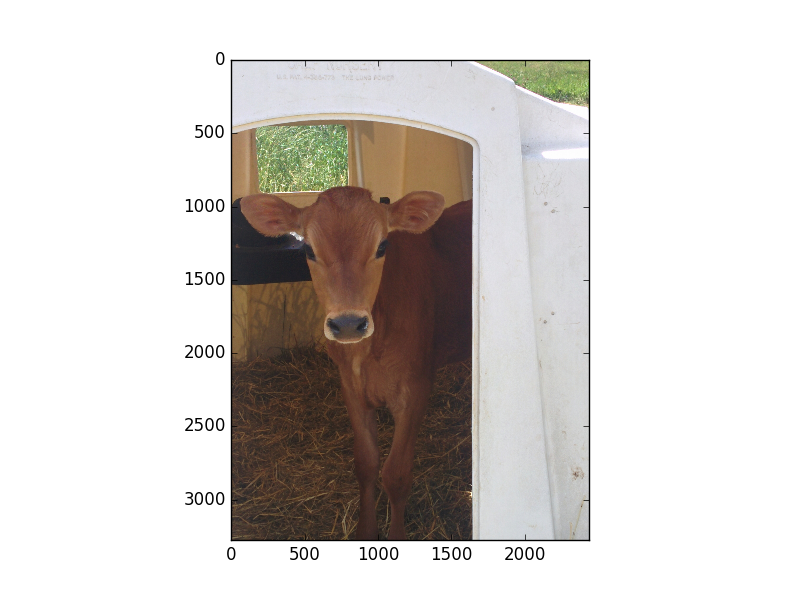
\includegraphics[width=1.1in]{calf_original}%
\caption{An image of a calf. This and corresponding images were created by the author.}
\end{figure}
%
% An example of a double column floating figure using two subfigures.
% (The subfig.sty package must be loaded for this to work.)
% The subfigure \label commands are set within each subfloat command, the
% \label for the overall figure must come after \caption.
% \hfil must be used as a separator to get equal spacing.
% The subfigure.sty package works much the same way, except \subfigure is
% used instead of \subfloat.
%%
\begin{figure}[H]
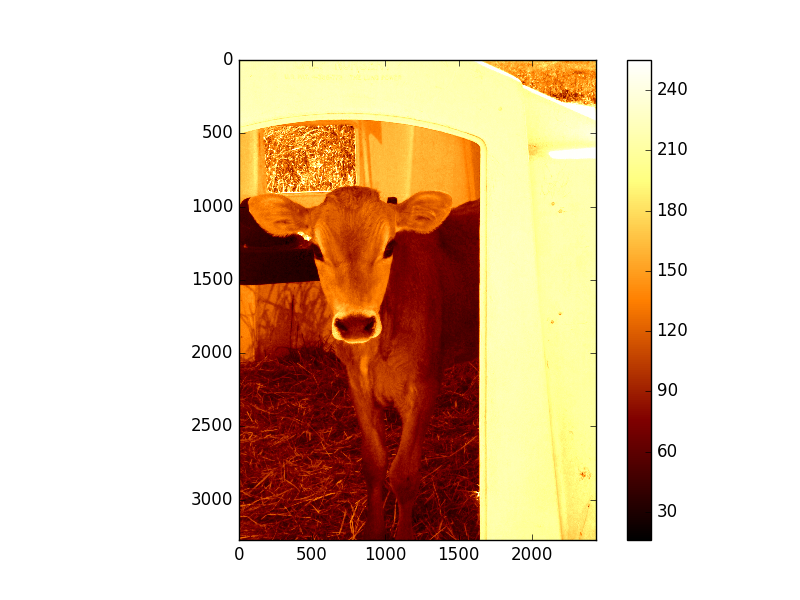
\includegraphics[width=1.1in]{calf_sequential}%
\hfil
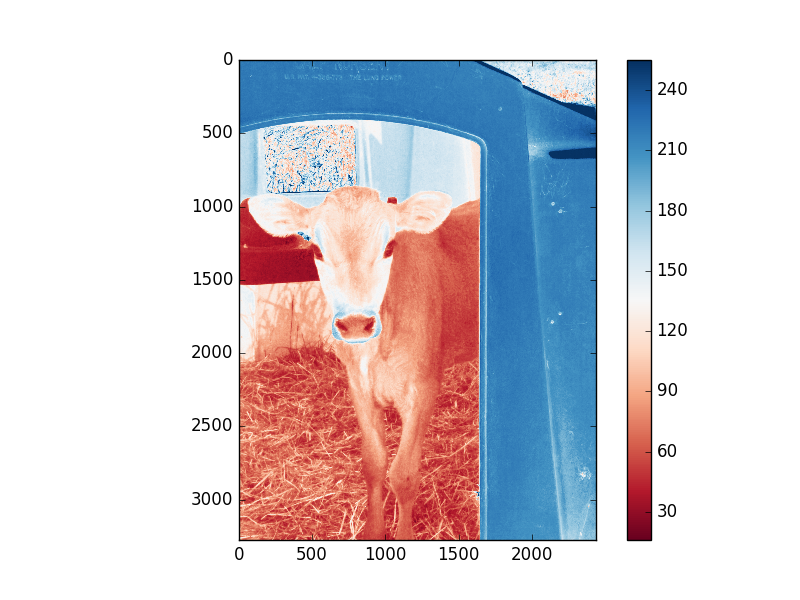
\includegraphics[width=1.1in]{calf_diverging}%
\hfil
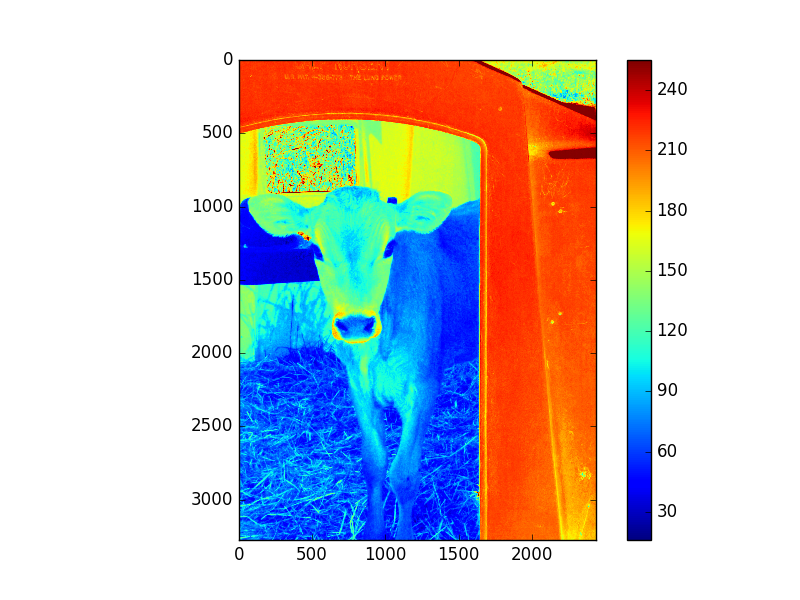
\includegraphics[width=1.1in]{calf_rainbow}%
\caption{The calf image plotted with a
sequential, diverging, and rainbow colormap.}
\end{figure}


\par
One advantage of the rainbow colormap is that it is easy to implement because it
is based on an older, simpler color model. Scientists use color models to understand
and work with color. These models are abstract mathematical representations that
describe a color as a collection of numbers that describe physical or perceptual
characteristics. These models have evolved to describe color specification systems,
color distance, and color appearance in different viewing conditions \cite{ciecam02}.
When a color model is used to produce color on a specific medium, the resulting set
of colors is called a color space. For example, the RGB model
describes color as the combination of red, green, and
blue light. A computer screen renders color using the
RGB model, thus the color produced by digital screens
with the RGB model is a color space. Another example is the
CMYK model, which describes color as combinations of
cyan, magenta, yellow, and black. Printers produce colors using this model.
\cite{colorimetry,colormapping}. The combination of cyan, magenta, yellow, and black
ink on a printer constitutes a color space. The selection and modification of color
models and spaces happens before colormaps or data visualizations can be created. 
\par
Most color spaces produce a similar set of colors. However, there are some colors
that do not translate well between color spaces. For example, consider the image
shown below. If you are reading this as a digital document, the colors will look
different than the colors on a printed copy of the same document. This represents
a transformation from an RGB color space to a CMYK color space \cite{colorvblackwhite}.
Color is lost in translation. This is the motivation for developing perceptually
uniform color models, as in the CIECAM02-UCS color model. Good models of color
distance may not preserve absolute color, but perceived color difference tends
to remain the same across all media \cite{ciecam02}. Perceptually uniform colormaps
can be produced using these models \cite{viridis}. In general, rainbow colormaps
are not perceptually uniform because the lightness is not consistent.
\par
This has not stopped some from attempting to modify---and therefore preserve---the
rainbow colormap. The adjustments refer to the Munsell color specification system,
which describes color with hue, saturation, and lightness. “This system
divides up the colors humans are capable of perceiving
into equal perceptual divisions of color lightness and
color saturation for each color hue. \cite{colormapping}”
Hue refers to the attribute generally associated with the color name (i.e. red,
orange, yellow, green, blue). On a color wheel, hue is the position of the color
on the color wheel. Saturation is the intensity of the hue. In
physical terms, it is the purity of the light wave frequency. Lightness is the
amount of light emitted by a color. Low lightness results in a darker color;
high lightness results in a lighter color. \cite{colorguidelines}.
Sisneros et al created a colormap modification framework that smooths the variation
in luminance (or lightness) and chromaticity, which is a combination of saturation
and hue. Their method can be applied to any perceptually non-uniform colormap.
However, their focus was on improving the rainbow colormap, since it is still widely
used in science. Their improved rainbow colormap contains subdued colors that better
represented image data \cite{chasingrainbows}. 
\par
Colors rendered in a color space are light waves---the
physical representation of color. These light waves are
interpreted by our brain when the light hits our eyes
\cite{viridis}. These light waves enter the human eye where
they hit the retina. The retina has two kinds of light
receptors, called rods and cones. Cones are more concentrated near the fovea centralis, the main focus point
of our eyes \cite{!SOURCE}. The cones capture red, green,
or blue light depending on the characteristics of each
cone. Rods do not interpret color \cite{colormapping}.

%\subsection{Choosing Colormaps}

\par
What are the criteria for evaluating a colormap? Several authors have created
methods to evaluate color
choice. In one paper, color schemes are evaluated by
three variables of the CIELUV color model. The first
is color distance. The CIELUV model is designed to
measure distance between colors. If the distances are
equally spaced, that’s a good thing. Linear separation
is the second variable. It refers to “the ability to separate targets
from non-targets in the colour model being
used.” For example, suppose a doctor wants to identify
a tumor and uses a colormap to display the data. If the
colors are not linearly sepparable in the color model, it
will be more difficult to identify the tumor even if the
colors are mathematically different. The third variable
is color category. This refers to color regions in which
there are both target and non-target elements \cite{colorchoice}.
 These characteristics do not account for multidimensional data projected into two-dimensional
space. CheckViz attempts to account for this problem
by using a perceptually uniform color coding so that
distortions such as those described above are accounted for when 
scientists want to visualize multidimensional data \cite{checkviz}.
The specific criteria of the color
model and color space must reflect the attributes of the colormap.
\par
Sometimes, when color encodings are converted to
grayscale, it can alter the perception of the data. There
are many algorithms to cast a color encoding to grayscale.

\subsection{Rainbow Colormaps}

There are multiple advantages to using rainbow colormaps. For one,
it is clear that users tend to prefer it
over other colormaps for its aesthetic appeal
\cite{spectralschemes, choropleth, endofrainbow}. 
The variety in hue also can accentuate relationships in the data than
a sequential, single-hue colormap. History is an advantage.
\par
However, the advantages can also be disadvantages.
When accentuating relationships, a human interpreter
might see signal where there is none. This seems to be
what happens when the data lie in certain regions (as in
between blue green and yellow) \cite{colorchoice}.
\par
Readers of scientific literature will recognize the rainbow colormap. 
It appears often in scientific publications and has 
broad appeal in the scientific community
\cite{endofrainbow, rainbowstill, spectralschemes,mapchoropleth}.
 Historically, rainbow colormaps like
MATLAB’s ‘jet’ have been the default colormaps used
in data-handling software \cite{matlab}. Despite its prevalence, 
many scientists oppose rainbow-gradient representations of data
\cite{rainbowstill, endofrainbow, viridis,arteryvis}.
 In one study, medical students were
asked to identify risk factors for heart disease in visualizations
of artery data. On average, the participants
using rainbow-colored visualizations took more time
and made more errors than participants using divergence-colored visualizations. 
Furthermore, the participants “thought they did well using the rainbow color
map even when in reality they did not perform as well
as the participants who used the diverging color map
\cite{arteryvis}.” This compelling evidence suggests
that the rainbow colormap is clearly inferior to other
colormaps.
\par
Others disagree. They claim that users have learned to
read data with the rainbow colormap and prefer its
aesthetic appeal \cite{spectralschemes, choropleth}. One
experiment tested data interpretation accuracy under
diverging, sequential, and spectral (rainbow) color
schemes. “Of 63 subjects who evaluated spectral and
sequential schemes, 56 percent selected spectral as the
best...We had expected the spectral scheme to interfere
with map-reading accuracy and with understanding
map patterns, but this did not occur,” Brewer writes.
“Our subjects preferred the spectral scheme
and performed well with it \cite{spectralschemes}.”
 While the rainbow colormap did not outperform other colormaps, it
appears to do no harm. Users can accurately interpret
rainbow-colored data visualizations.

\section{Color Perception and Color Vision Impairment}

One of the advantages of using perceptually uniform colormaps is
that they show the data accurately even if the colors do not appear
the same. Color perception can change for a number of reasons. When 
colors are placed near each other, it changes the way our eyes see that color.
The brain adjusts the amount of light that enters the eyes based
on external conditions. For example, colors appear more bright under diffused
light. Competing bright colors also diminishes the overall perception
of their brightness.

Mark Rothko and Josef Albers are notable artists who explored the human relationship
with color perception. Some colors blend together while others almost appear to be in
conflict with each other, causing a perceived vibration in the colors.

Another example of color perception under different conditions is the 
color-of-the-dress meme that became popular in 2015. The picture was
sent on social media sites asking whether the dress was black and blue
or white and gold. This effect happens because our eyes perform a kind 
of normalization under different light conditions. This adjustment alters
the perception of what the colors look like. Other examples from psychology 
place the same color in two images with different colors surrounding the
color being studied. Even though the colors are the same, they appear to be 
different because of the context that they are in. This means that sometimes
we see color differences even when there are none.

Other times, color differences can't be detected easily or at all. This is 
especially common among people who have some form of color vision impairment,
as in colorblindness. The estimated colorblind population is somewhere around 5-8\%
and affects mostly males of European descent.

Colorblindness results in colors falling on confusion lines---lines in which it
is difficult or impossible to distinguish between two colors. People with full
color vision also have confusion lines and so in some sense are colorblind because 
we can't see the entire spectrum of light as colors. However, color deficient viewers
are special in that they do not see the normal range of colors as their peers.
There are multiple kinds of colorblindness.
Full color deficiency results in black and white vision and is very rare.
The most common form of color deficiency results in confusing shades of red and green.
An example of a map colored with bright orange and green and what a deutoronome
would see is given in Figure 3.

For these genetic color deficiencies, it seems reasonable to design data
visualizations with colorblindness in mind. Unfortunately for the rainbow colormap,
the colors that a colorblind user sees are not the same as those seen by a person
with full color vision. Especially for high values, which are displayed in reds,
the variation in green is not easy to interpret for colorblind viewers. In fact,
though they are aesthetically pleasing, people are slower at interpreting data with
large variations in color and make more errors. Yet, colorblind people still seem
to get by fine.

Color deficient viewers use clues to distinguish between colors that easily confuse them.
Brewer has conducted extensive research into how color deficient
viewers interpret color-encoded information. She has suggested several ways in which 
maps and information visualizations can be designed to help color deficient viewers.
A common theme in her research, as well as others, is that colormaps are greatly
improved when the dark-to-light variation is controlled and used to show progression.
This is the idea behind perceptually uniform colormaps. Even when converted to black
and white, the visuals still preserve the nature of the data and are easy to interpret.



%
%[mapcvi]
%[mapchoropleth]
%[simultaneouscontrast]
%[ciecam02]
%[mapguidelines]
%[colorvblackwhite]
%[colormapping]

\section{Applications}
Use of color in data visualization extends to multiple
industries and disciplines. Foremost among these are medical imaging
and cartography. including engineering, med-
icine, statistics, computer science, graphic design, and
psychology \cite{colorguidelines}.
[arteryvis]
[standardizemedimg]
[visvars]
[mapchoropleth]

\section{Conclusion}
\blindtext[1]

\ifCLASSOPTIONcaptionsoff
  \newpage
\fi



% trigger a \newpage just before the given reference
% number - used to balance the columns on the last page
% adjust value as needed - may need to be readjusted if
% the document is modified later
%\IEEEtriggeratref{8}
% The "triggered" command can be changed if desired:
%\IEEEtriggercmd{\enlargethispage{-5in}}

% references section
%\bibliography{IEEEabrv,../bib/paper}
\bibliographystyle{ieeetr}
\bibliography{litreview}

% that's all folks
\end{document}



